\subsection{Scan}
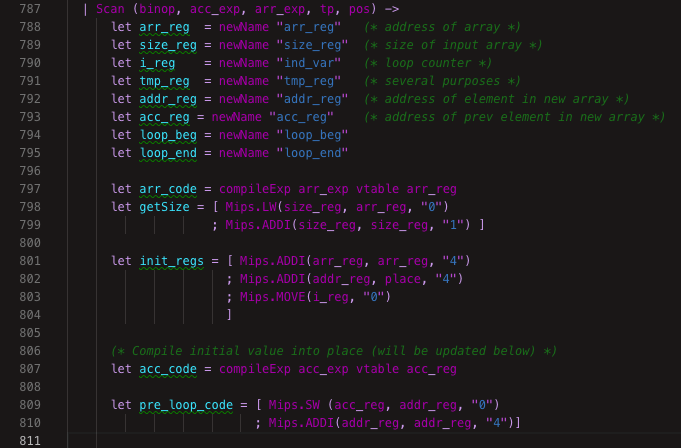
\includegraphics[width=\linewidth]{Materials/CodeGen/Scan1}
To implement Scan we first evaluate the input array, then we create a new array of size 'input\_array\_size + 1' to make space for the initial value (lines 804-805). Next we evaluate the accumulator expression. In the pre\_loop\_code the initial value of the accumulator is saved in the new array (lines 815-816).\\
The idea is we create a register to hold the accumulated value. Then we create a loop in where we apply the supplied function on the value in the accumulated register and the element in the input array and we save the value in the accumulated register. Then we save the value in the accumulated register in the new array and we begin the loop anew.
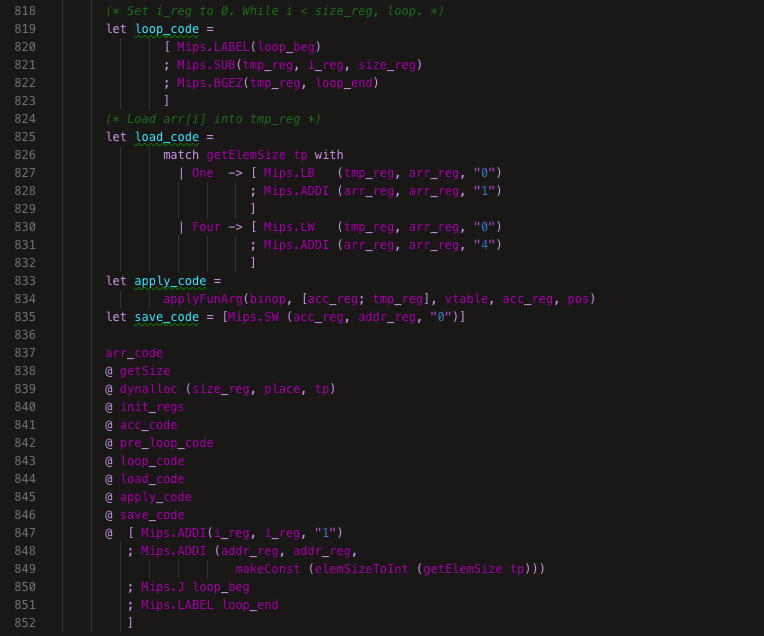
\includegraphics[width=\linewidth]{Materials/CodeGen/Scan2}
After we have tested whether the loop should terminate, we load the value of the input array into a temporary register (lines 825-832). We then apply the input function on the temporary register and the accumulator register and save the result in the accumulator register (lines 833-834). Lastly we save the value of the accumulator register in the new array and updates 'addr\_reg' to point to the next entry in the new array and we update 'i\_reg' and begin the loop anew.